\section{Задание 4. Работа с файловой системой.}

Файловый менеджер и основные операции с ним \ref{fig:createDir}, \ref{fig:useDir}, \ref{fig:delDir} :

\begin{figure}[!h]
    \centering
    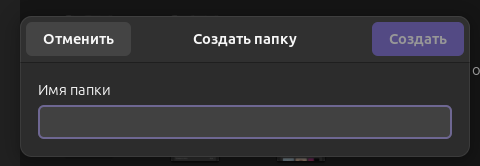
\includegraphics[width = 0.8\textwidth]{images/createDir.png}
    
    \caption{Создание папки}
    
    \label{fig:createDir}
\end{figure}

\begin{figure}[!h]
    \centering
    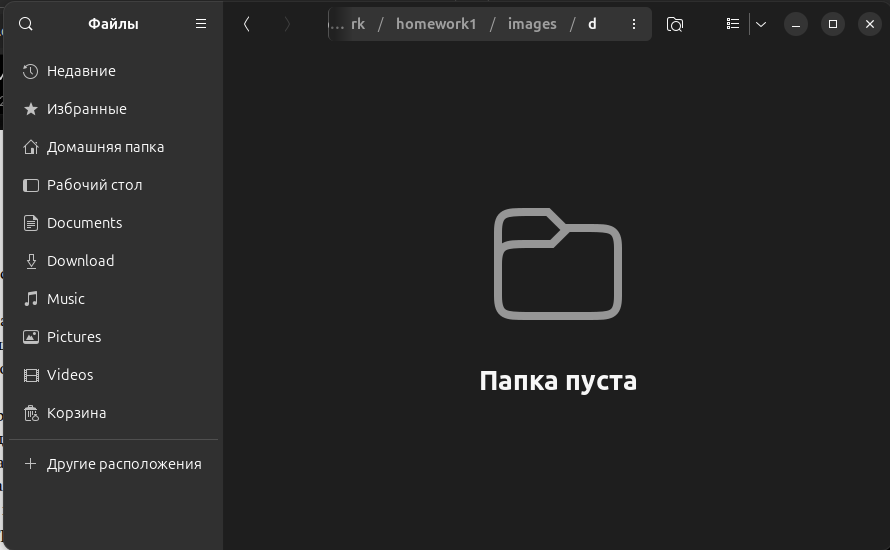
\includegraphics[width = 0.7\textwidth]{images/useDir.png}
    
    \caption{Действия с папкой + открытие папки}
    
    \label{fig:useDir}
\end{figure}

\begin{figure}[!h]
    \centering
    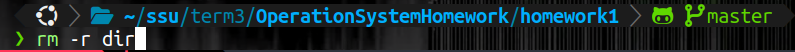
\includegraphics[width = 0.8\textwidth]{images/delDir.png}
    
    \caption{Удаление папки}
    
    \label{fig:delDir}
\end{figure}

\newpage

Структуры файловой системы ОС Ubuntu \ref{fig:homeDir}, \ref{fig:korenDir}, \ref{fig:usrDir} :

\begin{figure}[!h]
    \centering
    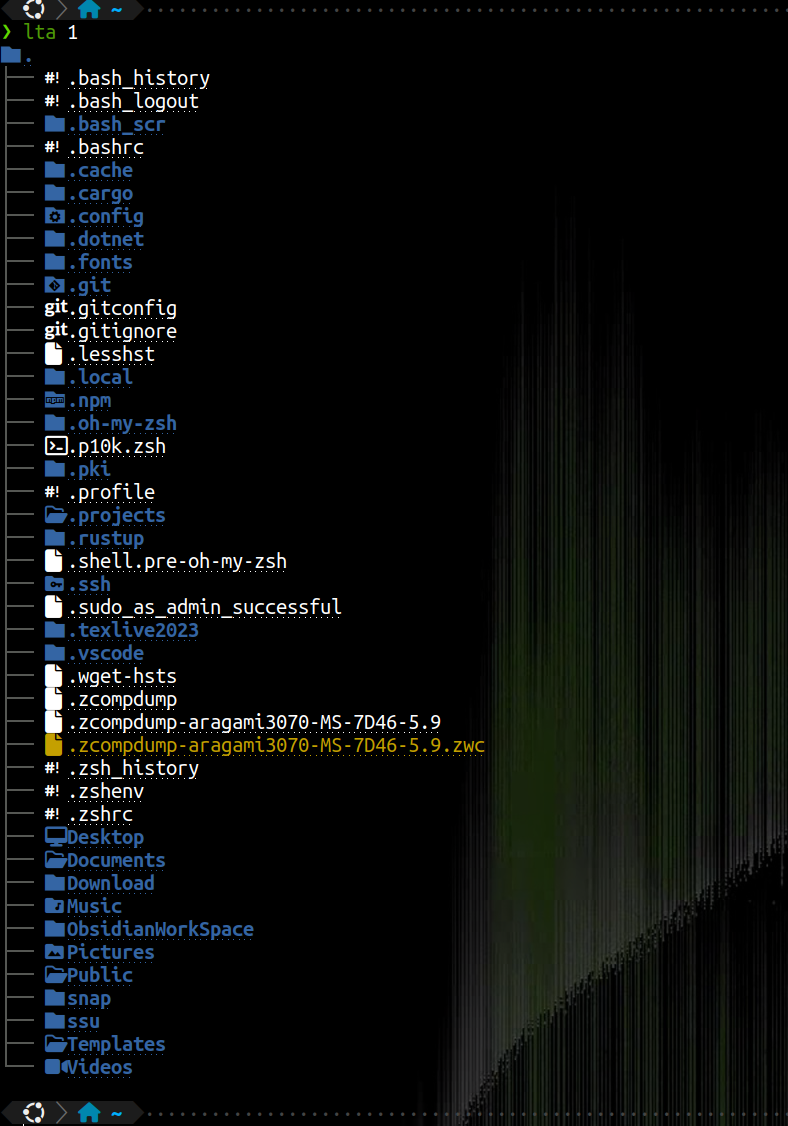
\includegraphics[width = 0.8\textwidth]{images/homeDir.png}
    
    \caption{Структура домашней директории}
    
    \label{fig:homeDir}
\end{figure}

\begin{figure}[!h]
    \centering
    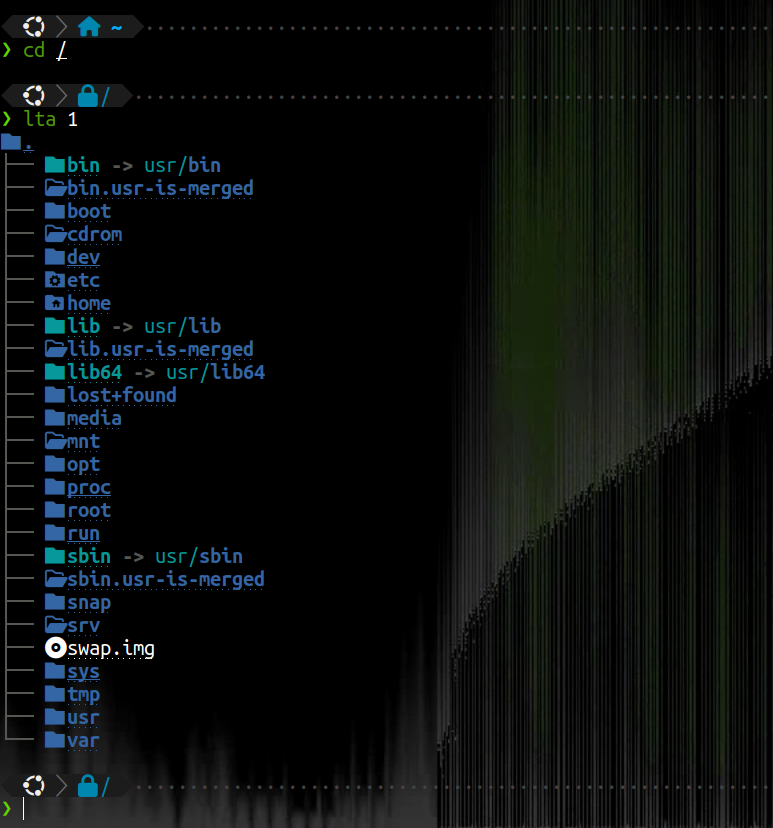
\includegraphics[width = 0.7\textwidth]{images/korenDir.png}
    
    \caption{Структура корневой директории}
    
    \label{fig:korenDir}
\end{figure}

\newpage

\begin{figure}[!h]
    \centering
    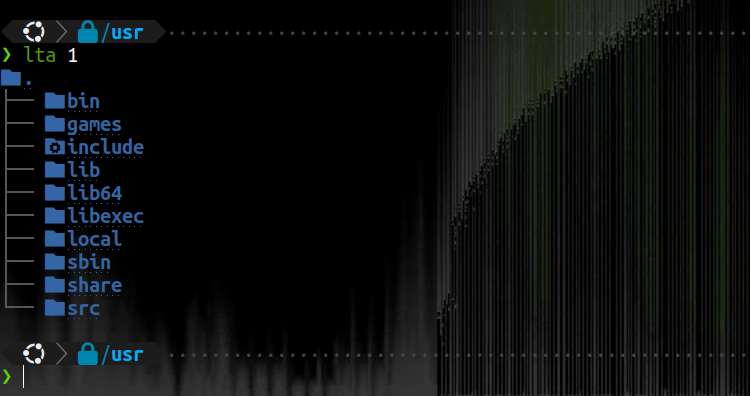
\includegraphics[width = 0.8\textwidth]{images/usrDir.png}
    
    \caption{Структура usr директории}
    
    \label{fig:usrDir}
\end{figure}
